\subsubsection{Typ}
Fristående program som förbehandlar testbeställarens applikation, och länkar samman denna med projektets moduler.

\subsubsection{Syfte}
Att snabbt och enkelt kunna integrera SuperRecorder SDK i ett nuvarande projekt för Android. Syftet relaterar direkt till URD 3.2.1.

\subsubsection{Funktionalitet}
Det finns två olika sätt som komponenten kan fungera på. Antingen är komponenten i form av ett mindre program, som testbeställaren laddar ner på sin egen dator. Programmet söker då igenom testbeställarens källkod, och modifierar den för att passa med projektets moduler. Kompilering sker sedan som vanligt, och applikationen skickas ut till testarnas mobiltelefoner. 

Ett annat alternativ är att länka samman testbeställarens applikation med SuperRecorder SDK efter kompilering. Detta sker genom så kallad dekompilering, för vilket verktyget \textit{apk-tool} är skapat. Om detta alternativ väljs skulle testbeställaren istället kunna skicka den kompilerade Android-applikationen till TBF:s servrar, där applikationen integreras med SuperRecorder och sedan skickas ut till testarna.

\subsubsection{Underordnade komponenter}
Komponenten har inga underordnade komponenter.

\subsubsection{Beroenden}
Verktyget \textit{apk-tool} och/eller lämpligt verktyg för automatiserad textbehandling.

\subsubsection{Gränssnitt}
Komponenten anropas en gång innan SuperRecorder kan exekvera, och har sedan inget gränssnitt mot det övriga systemet. 

\subsubsection{Resurser}
Komponenten behöver hela källkoden för den Android-applikation som ska testas, alternativt en kompilerad version av Android-applikationen i körbar form.

\subsubsection{Referenser}
Komponenten använder sig eventuellt av \textit{apk-tool}. Dokumentation finns på \url{https://code.google.com/p/android-apktool/}.

\subsubsection{Process}
Processen är en sekventiell genomgång av källkod eller dekompilerad Android-bytekod. På ett antal ställen i koden läggs nya instruktioner till som anropar SuperRecorders programmoduler. Programmet kompileras om. Om allt gått väl är filen redo att användas på testarnas mobiltelefoner. Har ett fel uppstått redovisas detta för testbeställaren, som i sådana fall hänvisas till en manuell kodintegrering.

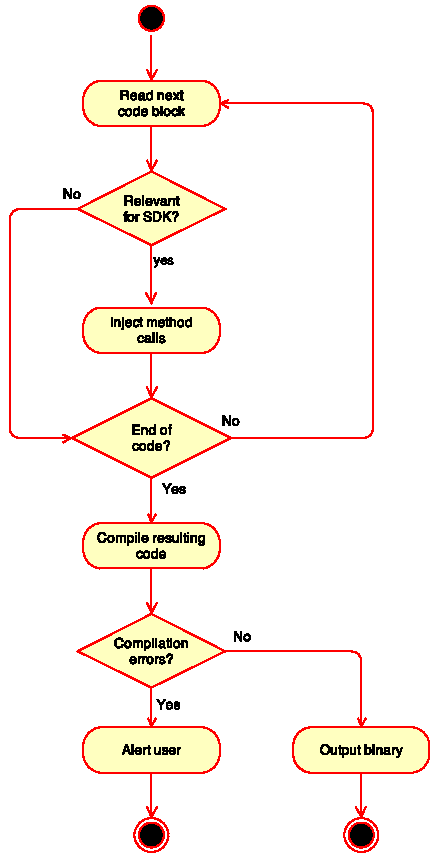
\includegraphics[scale=1.0]{integrateState.pdf}

\subsubsection{Data}
Komponenten behöver inte spara någon lokal data, utan använder sig bara av fördefinierade konstanter för att ändra på rätt delar av koden.
